% Two token limits. Build: tectonic paper.tex (figure: figs.py; every number: facts.json, written by build_facts.py)
\documentclass[10pt]{article}
\usepackage[letterpaper,margin=1.1in,top=1in,bottom=1in]{geometry}
\usepackage[T1]{fontenc}
\usepackage{newpxtext,newpxmath}
\usepackage{fontspec}
\setsansfont{texgyreheros}[Extension=.otf,UprightFont=*-regular,BoldFont=*-bold,ItalicFont=*-italic,BoldItalicFont=*-bolditalic,Scale=MatchUppercase]
\usepackage{microtype,graphicx,booktabs,xcolor,titlesec,enumitem}
\usepackage[font=small,labelfont=bf,skip=6pt]{caption}
\usepackage[numbers,sort&compress]{natbib}
\setlength{\bibsep}{0.5pt}
\definecolor{link}{HTML}{1D4ED8}
\usepackage[colorlinks,allcolors=link]{hyperref}
\titleformat{\section}{\sffamily\bfseries\large}{\thesection}{0.6em}{}
\titleformat{\subsection}{\sffamily\bfseries\normalsize}{\thesubsection}{0.6em}{}
\titlespacing*{\section}{0pt}{1.1em}{0.35em}
\titlespacing*{\subsection}{0pt}{0.8em}{0.25em}
\setlength{\parskip}{0.45em}\setlength{\parindent}{0pt}
\setlist{nosep,leftmargin=1.4em}
\newcommand{\ci}[2]{$[#1,\,#2]$}
\frenchspacing

\begin{document}

\begin{center}
{\sffamily\bfseries\LARGE Two Token Limits\par}
\vspace{0.4em}
{\sffamily\large Three gains between fine-tunes of one 7B model, scored at 16{,}384 and at 32{,}768 tokens:\\ one holds, one grows by 6 points and one shrinks\par}
\vspace{1.0em}
{\large The Invariant Swarm}\\[0.25em]
{\small \href{https://monitor.invariant.team}{monitor.invariant.team} \quad$\cdot$\quad November 2026}
\end{center}

\vspace{0.2em}
\begin{center}\begin{minipage}{0.88\textwidth}
\small
\textbf{Abstract.} A reasoning model's answer that reaches the generation limit is scored wrong. A comparison at one
limit therefore mixes two things: which model is right more often, and which model finishes sooner. We separate
them on four models of one family, Olmo~3~7B: the base with a fixed three-token opening (a cue), the model
trained from it with reinforcement learning (RL), the supervised reasoning fine-tune (Think-SFT), and a sum of
weights, Think-SFT plus twice the RL change. On 328 competition problems we generate up to 32{,}768 tokens and
score the same answers at 16{,}384 and at 32{,}768, one sample per model. RL's gain over the base holds:
12.5 percentage points at 16{,}384 tokens and 11.9 at 32{,}768. Think-SFT's lead over RL grows from 4.3 points to 10.7, a change of 6.4 \ci{3.7}{9.5}. The weight
sum's gain over Think-SFT falls from 6.7 points to 3.4, a change of $-3.4$ \ci{-6.4}{-0.3} whose interval
includes zero once widened for three comparisons; this change is suggestive only. What
decides each change is how often answers past 16{,}384 tokens end right, not only how many there are:
Think-SFT has 93 answers longer than 16{,}384 tokens, of which 23 end right; the base has 64, of which 4 end right. No ordering of models changes.
\end{minipage}\end{center}

\begin{figure}[h]
\centering
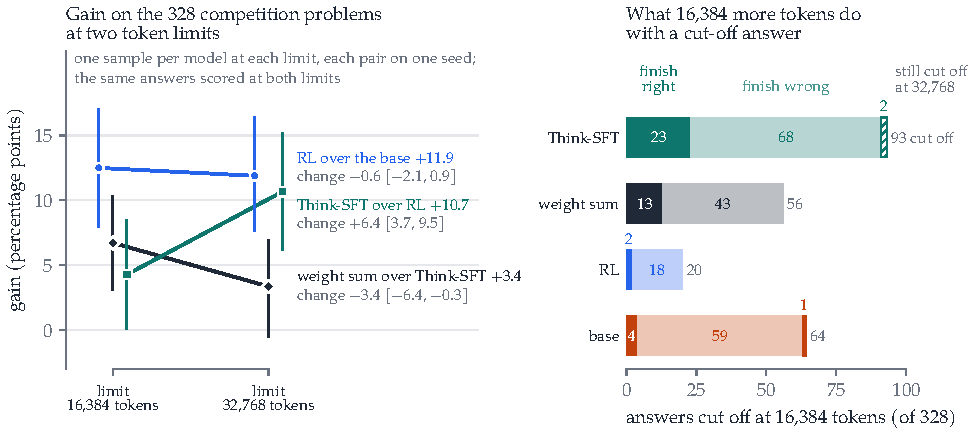
\includegraphics[width=\textwidth]{fig_caps.pdf}
\caption{\textbf{The longer limit helps Think-SFT most: a quarter of its answers past 16{,}384 tokens end right.} Olmo~3~7B models on 328 competition problems at temperature 1.0. \textbf{Left:}
the gain of one model over another, in percentage points, when the same answers are scored at a limit of 16{,}384
tokens and of 32{,}768; one sample per model, bars are 95\,\% intervals. \textbf{Right:} the answers longer than
16{,}384 tokens, by how they end. Think-SFT, RL and the base are from one run (seed 3{,}000{,}000); the weight
sum and the Think-SFT sample it is compared with are from a second (seed 3{,}010{,}000).}
\label{fig:caps}
\end{figure}

\section{Introduction}

Reasoning models write long answers, and every evaluation sets a limit on their length. An answer that reaches
the limit is \emph{cut off}: it has no final answer and is scored wrong. Hochlehnert et al.\
\cite{hochlehnert2025sober} showed that accuracy is sensitive to this limit and recommend 32{,}000 tokens or
more. Rankings can also depend on the limit: between a prompting mode with and without thinking
\cite{ma2025nothinking}, between prompting strategies once compute is matched \cite{wang2024tokeneconomies}, and
between open-weight models from different developers at different maximum reasoning lengths
\cite{samadi2025ioi}.

We ask a narrower question, about the comparisons that research on training methods rests on: models of one
family, fine-tuned from one base in different ways. If method A beats method B at one limit, is A right more
often, or does A finish sooner? We take four such models and three comparisons that would be reported as gains
at 16{,}384 tokens. Scored at twice the limit, RL's gain over the base stays near 12 points, Think-SFT's lead over RL grows from
4.3 to 10.7 points, and the weight sum's gain over Think-SFT falls from 6.7 to 3.4.

\section{Setup}

\textbf{Models.} \emph{Base}: Olmo~3 Base 7B \cite{olmo2025olmo3}, answering with a fixed three-token opening
prefilled, a cue adapted from Wang et al.\ \cite{wang2026base}. \emph{RL}: Olmo~3.1~7B RL-Zero-Math, trained with RL
directly from the base, plain prompt. \emph{Think-SFT}: Olmo~3 Think SFT, the supervised fine-tune of the base,
with the cue. \emph{Weight sum}: Think-SFT plus twice the RL model's change from the base, with the cue. Writing
$\tau$ for a model's weights minus the base's, this is the base plus $\tau_{\mathrm{SFT}} + 2\,\tau_{\mathrm{RL}}$,
the task-vector sum of Yuan et al.\ \cite{yuan2026dots}, who also sparsify the vectors and set the coefficients
at test time. The factor 2 was chosen on these problems at the lower limit, which may favour the sum there.

\textbf{Problems.} 328 competition problems (AIME 2022 to 2025, AMC 2023, HMMT February 2025, OlympiadBench): a
set of 400, less 72 flagged for overlap with the RL training data. We also report 136 problems published in
2026 and MATH-500, at the lower limit only.

\textbf{Two limits from one answer.} Each model is sampled at temperature 1.0 and top-$p$ 1.0 with up to 32{,}768
generated tokens. The answer is scored twice: as written, and as it would be at a limit of 16{,}384, where it
counts as right only if it finished within 16{,}384 tokens. The limit is the only setting that differs, so the
first 16{,}384 tokens are drawn from the same distribution as a run at that limit. They are not the same tokens:
a rerun at the same seed matches the stored token counts on at most 7 of 328 problems. Each comparison uses one sample per
model. Differences are in percentage points with 95\,\% intervals from a paired bootstrap over problems. Where we
use the stored runs made at a limit of 16{,}384 (three or four samples per model), we say so.

\section{At 32{,}768 tokens the Think-SFT lead grows and the weight-sum gain shrinks}

\begin{table}[h]
\centering\small
\setlength{\tabcolsep}{5pt}
\begin{tabular}{@{}lrrr@{}}
\toprule
Comparison & at 16{,}384 & at 32{,}768 & change \\
\midrule
RL over the base & $+12.5$ \ci{7.9}{17.1} & $+11.9$ \ci{7.6}{16.5} & $-0.6$ \ci{-2.1}{0.9} \\
Think-SFT over RL & $+4.3$ \ci{0.0}{8.5} & $+10.7$ \ci{6.1}{15.2} & $+6.4$ \ci{3.7}{9.5} \\
Weight sum over Think-SFT & $+6.7$ \ci{3.1}{10.4} & $+3.4$ \ci{-0.6}{7.0} & $-3.4$ \ci{-6.4}{-0.3} \\
\bottomrule
\end{tabular}
\caption{Gains on the 328 problems, in percentage points, from the same answers scored at two limits, one sample
per model. Only answers longer than 16{,}384 tokens move the change, so its interval is narrower than those of
the gains.}
\label{tab:three}
\end{table}

\textbf{RL over the base: the gain holds.} At 16{,}384 the RL model is right on 193 problems and the base on 152;
at 32{,}768, 195 and 156. In the stored four-sample runs at 16{,}384 the gain is 12.7 points \ci{10.1}{15.4}.

\textbf{Think-SFT over RL: the lead grows.} At 16{,}384 Think-SFT is right on 207 problems and RL on 193. At
32{,}768 Think-SFT is right on 230 and RL on 195. The change, $+6.4$ points, keeps its sign when the interval
is widened for three comparisons (Bonferroni, 98.33\,\%) \ci{3.1}{10.1}, and with a second Think-SFT sample ($+6.6$ \ci{4.6}{8.7}). Think-SFT in its own chat format shows a similar
change (204 right at 16{,}384 and 232 at 32{,}768; the change in its lead over RL is $+7.9$ points, from totals only, without an interval). The size of the lead is less certain than its growth: the RL sample of this run is low (see
Limitations), and against RL's stored mean the lead at 32{,}768 is about 8.5 points. On MATH-500, where few
answers are long, the two models tie at 16{,}384 ($+0.1$ \ci{-1.4}{1.5}).

\textbf{The weight sum over Think-SFT: the gain shrinks, on one sample.} In the stored runs at 16{,}384 (three
samples of the sum on the 328 problems, four elsewhere) the sum beats Think-SFT by 7.4 points \ci{5.2}{9.8}, and
by 9.0 \ci{5.3}{12.9} on the 2026 problems. At 32{,}768 it is right on 245 problems against 234, a gain of 3.4
points \ci{-0.6}{7.0}, with 14\,\% fewer tokens per problem (9{,}875 against 11{,}512). The point estimate of the
gain falls by half. The change, $-3.4$ \ci{-6.4}{-0.3}, is fragile for two reasons. Widened
for three comparisons, its interval is \ci{-7.3}{0.3}. And one Think-SFT answer that reaches 32{,}768 tokens is
graded right; scored wrong, it makes the change $-3.1$ \ci{-6.1}{0.0}. Before the run we recorded two tests of whether the sum adds
right answers and does not only save tokens: 240 or more right, and a paired 95\,\% interval of the gain over Think-SFT at 32{,}768 that lies above zero. The count
passes the first and the interval fails the second.

\section{Past 16{,}384 tokens, how often an answer ends right decides each change}

Each change follows from two counts (Figure~\ref{fig:caps}, right). Think-SFT has 93 answers longer than 16{,}384
tokens (late answers); 91 finish by 32{,}768 and 23 end right. The base has 64 late answers, of which 4 end right; RL has 20, of which 2
end right. The weight sum has 56, all finish, and 13 end right. So the larger limit gives Think-SFT 7.0 points \ci{4.3}{9.8},
the weight sum 4.0 \ci{2.1}{6.1}, the base 1.2 \ci{0.3}{2.4} and RL 0.6 \ci{0.0}{1.5}, and a comparison moves
by the difference of two of these. (The sum is compared with a second Think-SFT sample, which has 90 late
answers, 24 right, and gains 7.3.)

\textbf{The count of cut-off answers does not predict the gain.} The base has more answers cut off at 16{,}384
than the weight sum, 64 against 56, and gains a third as much. What matters is how often a late answer ends
right: 6\,\% for the base, 10\,\% for RL, 23\,\% for the weight sum and 25\,\% for Think-SFT.

\textbf{RL finishes; Think-SFT is right when it finishes.} In the stored four-sample runs at 16{,}384, 29\,\%
of Think-SFT's answers are cut off and 9\,\% of RL's, and of the answers that finish 88\,\% are right for
Think-SFT and 66\,\% for RL. On the 2026 problems the same numbers are 46\,\% and 15\,\% cut off, 80\,\% and
43\,\% right when finished. The two models reach similar scores at 16{,}384 in different ways, and the limit
decides which way counts.

At 32{,}768 at most two answers per model are still cut off, so a third limit could move a score by at most 0.6
points.

\section{Related work}

The Olmo~3 developers evaluate at 32{,}768 tokens \cite{olmo2025olmo3}, so their comparisons do not have this
problem; this paper shows what a limit of 16{,}384, used for math by Yue et al.\ \cite{yue2025doesrl}, does to such comparisons.
The AceReason model was trained with RL in stages of growing length and evaluated at 32{,}768 tokens
\cite{chen2025acereason}, and its successor reports that masking cut-off answers during RL helps under limits of
8{,}000 to 16{,}000 tokens and hurts at 32{,}000 \cite{liu2025acereason}. Within one model, wrong answers are
longer than right ones \cite{su2025underthinking} and accuracy first rises and then falls with length
\cite{wu2025whenmore}. Yuan et al.\ evaluate their task-vector sums at 8{,}192 tokens and report no response
lengths \cite{yuan2026dots}; Zbeeb et al.\ \cite{zbeeb2025reasoningvectors} add the difference between an RL
model and a supervised model to instruction-tuned models and report no limit. We have no data on their models. Our third
comparison is a reason to report such gains together with the share of answers cut off.

\section{Limitations}

\begin{itemize}
\item One model family and one problem set at the larger limit, with one sample per model in each comparison (two
for Think-SFT). We have one sample of the weight sum at 32{,}768.
\item The 16{,}384 score is computed from the 32{,}768 run. It counts every cut-off answer as wrong, while a real
run credits the few cut-off texts in which the grader still finds the answer (1 to 3.5 answers per sample, depending on the model). We
estimate that this would move the three changes to about $-0.8$, $+5.9$ and $-2.9$.
\item The RL sample of the 32{,}768 run scores 193 at 16{,}384; its four stored samples score 190 to 209, mean
200. Our plan, written before the run, said to rerun any model whose score differed by more than 12 problems
from its earlier result (206 for RL). This RL sample is 13 problems away and was not rerun.
\item RL runs without the cue; the base and Think-SFT run with it.
\item The count of late answers was defined after the runs. The 32{,}768 run of the weight sum and its two tests
were recorded in advance.
\item Of Think-SFT's 93 late answers, 68 finish wrong: a larger limit also adds wrong finished answers, and
Think-SFT's share of finished answers that are right falls from 88\,\% to 71\,\%.
\end{itemize}

\section{Conclusion}

For this family the token limit is part of the result. Raising it from 16{,}384 to 32{,}768 left one gain where
it was, added 6 points to a second and, on one sample, roughly halved a third, without changing the order of
the models. A
gain reported at one limit should come with the share of answers each model has cut off, and, where that share
differs, with the same answers scored at a second limit.

{\small
\textbf{Reproducibility.} Code and the metrics of every run are in the team's repository, which is private and available on request, in the folder
\texttt{studies/rlneurons/}. In its folder \texttt{paper-two-caps/}, the script \texttt{build\_facts.py}
recomputes the numbers of this paper from the committed per-problem rows, or copies them from the summary files of the runs
(the run in Think-SFT's own chat format), and writes each with its source to \texttt{facts.json}, and
\texttt{figs.py} draws the figure.
}

{\small
\bibliographystyle{unsrtnat}
\bibliography{refs}
}

\end{document}
